Die Studie wurde im Rahmen des Verbundprojektes BACOSA (Baltic Coastal System Analysis and Status Evaluation) durchgeführt, bei dem in Zusammenarbeit der Universitäten Kiel, Rostock und Greifswald die Flachgewässer der südlichen deutschen Ostsee untersucht werden. Die Studie umfasst den Zeitrahmen April 2013 bis April 2016 und setzt sich zum Ziel, die Funktionen der Ökosysteme ausgewählter Buchten der Ostsee in einer möglichst umfassenden Gesamtheit zu verstehen, insbesondere die Auswirkung von Makrophyten auf die Sedimentdynamik und die Erfassung der Pelagial-Benthos-Wechselwirkung hinsichtlich der Stofftransporte. Außerdem werden auf Basis vorhandener Daten die Ökosystemdienstleistungen dieser Gewässer bewertet. 

Die Forschungsergebnisse sollen zum grundsätzlichen Verständnis der Ökosysteme beitragen und damit eine Grundlage zum Erfüllen der Forderungen der Europäischen Meeresstrategierichtlinie (EU-MSRL) und der Europäischen Wasserrahmenrichtlinie (EU-WRRL) schaffen. In dieser Diplomarbeit werden an zwei Standorten in den Boddengewässern Hiddensees und an weiteren vier Stationen an der südlichen deutschen Ostsee entlang des Salzgradienten die Vegetationsstruktur sowie Wechselwirkungen zwischen Makrophytobenthos und Sedimentstruktur charakterisiert. Zeitgleich und an den gleichen Probenahmestellen wurden das gelöste Sediment in der Wassersäule \citep{kafka_2014}, das Phytoplankton \citep{lindner_2014} und das Zooplankton \citep{nawka_2014} untersucht. Eine möglichst detailgenaue Beschreibung der Phytobenthos-Struktur in der Wassersäule soll auch eine Grundlage für die oben genannten Arbeiten schaffen.
\\
Das Makrophytobenthos der Ostsee ist der Bewuchs des Meeresbodens (des Benthals) mit Kormophyten (Seegras und brackwasserangepasste höhere Pflanzen) sowie mit makroskopischen Algen \citep{schwenke_1995}. Die Ostsee ist eines der größten Brackwassergebiete der Erde und erst vor etwa 12.000 Jahren entstanden. Sie ist, verglichen mit der Nordsee, artenarm, denn es gibt nur wenige echte Brackwasserorganismen. Die meisten Tier- , Pflanzen- und Algenarten sind über die Nordsee eingewandert \citep{rheinheimer_1995}. In küstennahen Bereichen mit Süßwassereinfluss finden sich auch limnische Arten, dazu gehören unter anderem alle in den Bodden der Ostsee vorkommenden Spermatophyten. Typische Vertreter sind zum Beispiel \textit{Myriophyllum spicatum}, \textit{Potamogeton pectinatus}, \textit{Zannichellia palustris} und \textit{Najas marina}. Sowohl die marinen als auch die limnischen Arten leben in der Ostsee an der Grenze ihres ökologischen Toleranzbereiches und reagieren empfindlich auf weitere Stressfaktoren \citep{rheinheimer_1995}.

Der Salzgehalt der Ostsee nimmt von Westen, wo der Einstrom über den großen Belt erfolgt, nach Osten hin ab. Gründe hierfür sind die Beckenbodenstruktur (durch Schwellen und Verengungen kann das salzige Tiefenwasser nicht frei zirkulieren) und die Süßwasserzuflüsse. Mit dem abnehmenden Salzgehalt sinkt die Diversität der marinen Arten, insbesondere nimmt die Anzahl der Brauntange stark ab \citep{schwenke_1995}. Viele marine Arten bilden Wuchsformen aus und werden kleiner mit abnehmendem Salzgehalt \citep{schwenke_1995}.

Das Makrophytobenthos ist ein wichtiger Bestandteil des Brackwasserökosystems. Beispielsweise produziert es Sauerstoff (im  Gegensatz zum Phytoplankton auch im bodennahen Bereich), es nimmt Nährstoffe aus der Wassersäule auf, die hierdurch für das Phytoplankton zeitgleich nicht zur Verfügung stehen, es bietet Laichorte für Fische und Versteckmöglichkeiten für Jungfische und Zooplankton und dient als Nahrung für phytophage Wasservögel.
Zudem können Pflanzen und Algen das Strömungsregime beeinflussen \citep{leonard_2006, li_2014, hurd_1997, siniscalchi_2012} und damit einen Einfluss auf die gelösten Partikel in der Wassersäule \citep{horppila_2003, leonard_1997, leonard_2006, ward_1984} und auf das Sediment \citep{madsen_2001} haben. 

\citep{madsen_2001} beschreibt die Interaktionen zwischen Phytobenthosbewuchs, Strömung und Sediment als ein sehr komplexes System mit gegenseitigen Einflussnahmen aufeinander (Vgl. Abbildung \ref{fig:schema_Makrophyten,Sedimente,Hydrodynamik}).


\begin{figure}[htb]
\centering
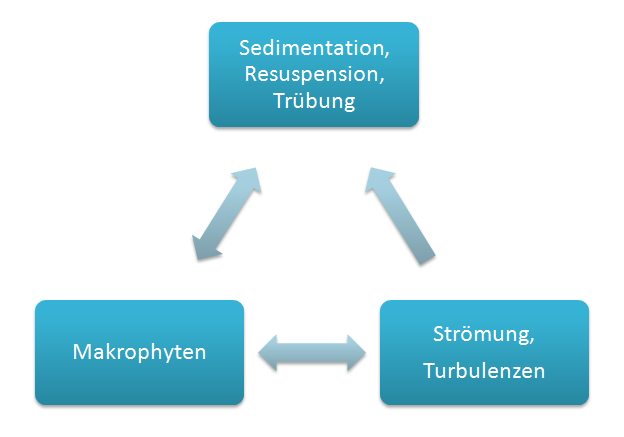
\includegraphics[width=0.68\textwidth]{images/Schema_Pfl_Sedim_Strm}
\caption[Zusammenhänge zwischen Makrophyten, Sediment- und Hydrodynamik]{Schematische Darstellung der komplexen Zusammenhänge zwischen Makrophyten, Sediment- und Hydrodynamik}
\label{fig:schema_Makrophyten,Sedimente,Hydrodynamik}
\end{figure}


Pflanzen haben einen Einfluss auf die Strömung, indem sie Schwingungen mit niedriger Frequenz (Large Scale Eddies) zu Schwingungen mit hoher Frequenz (Small Scale Eddies) umbrechen und damit Turbulenzen verursachen \citep{leonard_2006}. Außerdem wird die Strömungsgeschwindigkeit innerhalb eines Pflanzenbestandes mit zunehmenden Deckungsgraden herabsetzt, während sie oberhalb des Bestandes unverändert hoch bleibt \citep{li_2014}.

Die Strömungsgeschwindigkeit hat umgekehrt auch einen Einfluss auf das Makrophytenwachstum. So können starke Strömungen und Wellenschlag die Pflanzen mechanisch schädigen und wachstumsreduzierend wirken \citep{biggs_1996}. Strömung kann die Submersvegetation jedoch auch positiv beinflussen, so stellte \citep{madsen_1997} fest, dass die abgerissenen Sprossteile von \texit{Myriophyllum spicatum} wurzeln und sich auf diese Art eine vegetativ vermehren können. \cite{madsen_1983} fand auch heraus,  dass sich bei allgemein geringen Strömungsverhältnissen von \unit{0 bis 0,1}{\metre\per\second} eine leichte Erhöhung der Strömungsgeschwindigkeit  positiv auf Wachstum und Photosyntheserate der Pflanzen auswirkt.

Durch den oben beschriebenen Einfluss der Pflanzen auf die Strömung können Vegetationsbestände indirekt einen Einfluss auf das Sediment haben, denn die Strömung beeinflusst die Sedimentations- und Resuspensionsverhältnisse: 
Resuspension findet statt, wenn die für eine bestimmte Korngröße kritische bodennahe Strömungsgeschwindigkeit (friction velocity) überschritten wird. Dann geraten die Teilchen in Bewegung, lösen sich unter Überwindung von Schwerkraft, Reibung und Partikelanziehung aus dem Sediment (Erosion) und werden in der Wassersäule gelöst (Resuspension) \citep{madsen_2001, hartge_1991}. Die kritische Geschwindigkeit ist dann erreicht, wenn die Kräfte, die ein Korn oder ein Aggregat in seiner Lage halten (Schubwiderstandskräfte) kleiner werden als die Kräfte, die auf seine Verlagerung hinwirken. \cite{laenen_1996} zeigen, dass sich die für die Resuspension benötigte Kraft (Bodenschubspannung, Scherkraft) flächenbezogen für einen Punkt im Gewässer berechnen lässt als:

\begin{align*}
\tau &= \rho f u_{max}^{2} & \rho &=\text{Water density}\\ 
     &     				   &  f   &= \dfrac{1}{\text{Reynolds number}}\\
     &					   & u_{max} &= \text{Maximum bottom boundary velocity}.
\end{align*}


Die abhängigen Größen sind die Wasserdichte (Viskosität), die charakteristische Länge der Sedimentteilchen (Reynolds-Zahl) und die maximale Fließgeschwindigkeit an der Grenzschicht zwischen freiem Wasserkörper und Sediment. Diese Geschwindigkeit (u) kann berechnet werden als:

\begin{align*}
u_{max} &= \frac{\pi H}{T sinh (2 \pi h / L_{0})} & H &=\text{Wave height}\\ 
        &     				                     & h &= \text{Water depth}\\
        &										 & L &= \text{Wave Length}.
\end{align*}


Die Formel zeigt, dass auch die Wellenperiode, die Wellenlänge, die Wellenhöhe und die Wassertiefe eine bedeutende Rolle für die Resuspension spielen. Diese wiederum sind abhängig von der Windlauflänge (Fetch) und von der Windstärke (Vgl. \cite{laenen_1996} für Berechnungen von Fetch und Wellenparametern). Die Einberechnung der Fetch zeigt, dass die mögliche Resuspension auch abhängig von der geografischen Lage und der Exposition des Standortes ist. 

In Studien mit Seesedimenten im Strömungskanal konnte \cite{hu_2011} nachweisen, dass sich die Resuspension von freiliegendem, unbewachsenem Sediment mit steigender Strömungsgeschwindigkeit erhöht. 
Dass die Resuspension in Makrophytenbeständen geringer und die Resuspension höher sind als auf vegetationsfreien Flächen wurde bereits in limnischen Freilanduntersuchungen \citep{horppila_2003, horppila_2005} und in Buchten der Ostsee \citep{kaitaranta_2013} beobachtet. Der Anteil der Vegetation in der Wassersäule betrug in bei allen Studien zwischen \unit{30 bis 35}{\%}.

Neben der Tatsache, dass Makrophyten Turbulenzen erzeugen und die Wellenlänge reduzieren und insgesamt dazu in der Lage sind, Srömungsgeschwindigkeiten zu reduzieren (vgl. Ergebnisse der oben genannten Autoren), fangen sie selbst durch ihre Biomasse – durch die Stängel, Blattspreiten, Blattquirle bei den Spermatophyten und durch die Thalli bei den Makroalgen – feinstes Sediment (Silte und Feinsande) auf \citep{ma_2008}. 

\cite{ward_1984} sowie \cite{fonseca_1986} fanden in Studien im Freiland sowie im Strömungskanal zudem heraus, dass die Resuspension abhängig ist vom Anteil der Pflanzen an der Wassersäule. Die Strömungsgeschwindigkeiten wurden umso effizienter reduziert und das Material umso mehr akkumuliert, je höher der Anteil der Makrophyten an der Wassersäule war. 

\cite{madsen_2001} geht davon aus, dass sich die Makrophyten durch ihre Anwesenheit einen positiven Feedbackloop verschaffen, indem sie durch Steigerung der Sedimentation und die Reduzierung der Resuspension die Trübung vermindern und damit die Lichtverfügbarkeit am Grund zum Vorteil der eigenen Photosyntheseleistung erhöhen.

Es wurde beobachtet, dass sich in Makrophytenbeständen mehr organisches Material im Sediment befindet als im makrophytenfreien Bereich \cite{kenworthy_1982}. Erst bei starken Windereignissen kann es hier zu schlagartigen Resuspensionsereignissen kommen, bei denen das feine organische Material und damit Nährstoffe in die Wassersäule gelangen \citep{dauby_1995}, wodurch wiederum das Phytoplanktonwachstum angekurbelt werden kann \citep{cowan_1996}. 
Das Phytoplankton ist der bedeutendste Produzent organischer Substanz im aquatischen Milieu. Jedoch können die höheren Organismen des Makrophytobenthos ebenfalls Fotosynthese betreiben und unter Umwandlung von Sonnenenergie in chemische Energie Glucose und durch Polymerisation weitere, langkettige organische Stoffe aufbauen. Durch Absterbeprozesse und Stoffumwandlungen vor allem durch das Zoobenthos kann es in Makrophytenbesständen und in ihrer unmittelbaren Nähe zur Anreicherung der organischen Substanz an der Sedimentoberfläche kommen. Unter aeroben Bedingungen wird sie durch Mikroorganismen oxidiert und in ihre Bestandteile $ CO_2 $ und $ H_2O $ aufgespalten, unter anaeroben Bedingungen wird die organische Substanz nur unvollständig zersetzt und es reichert sich vermehrt an.
\\

Um herauszufinden, ob und in welcher Intensität typische Makrophytenbestände der Ostseebodden einen Einfluss auf das Sediment, seine mittlere Korngröße und Feinpartikelanteil sowie auf seinen organischen Gehalt haben, wurden Untersuchungen an 6 Standorten entlang der südlichen deutschen Küste durchgeführt.

Dabei wurden an jedem Standort zwischen dicht und spärlich bewachsenen Gruppen unterschieden und unterschiedliche Artenzusammensetzungen und Vegetationsstrukturen ausgewählt, darunter waren Grundrasen, dominiert von Angiospermen wie \textit{Ruppia sp}. und \textit{Zannichellia sp}. sowie von Makroalgen (\textit{Fucus vesiculosus f. balticus}), sowie gleichzeitig dicht und weit in die Wassersäule hineinreichende Seegrasbestände.

Von besonderem Interesse war die Wechselwirkung zwischen Sediment und Wasser in einem bisher in Bezug auf den Einfluss auf das Sediment und die Resuspension bisher überhaupt nicht untersuchten Ökosystem, einem dichten Bestand der Braunalge \textit{Fucus vesiculosus f. balticus}. 

Die meißten Ökosystem-Studien, die \textit{Fucus vesiculosus} -Habitate einschließen, beziehen sich auf die Braunalge als eine auf Steinen und Geröll im Brandungsbereich fest verankerte Alge.
In den Boddengewässern Hiddensees jedoch bildet sie eine unbewurzelte, dem Sediment aufliegende Kümmerform (f. balticus) aus \citep{k}(!Künzenbach, Müller-Stoll, Fluegge, eigene Beobachtung).  Diese ist taxonomisch keine eigene Art, sondern stellt nach genetischen Untersuchungen lediglich eine Wuchsform von \textit{Fucus vesiculosus} dar \citep{athanasiadis_1996} und siedelt typischerweise auf Sand und schlickigem Sand in geschützten Buchten bis maximal \unit{2}{\metre} Tiefe \citep{helcom_red_list_macrophyte_expert_group_2013} und kann bei ausreichenden Bodenschubspannungen verdriftet werden \citep{canal-verges_2010}.

Wie \cite{flugge_2004} bei Vegetationskartierungen in der Griebener Bucht bereits festgestellt hat, verändert sich sowohl die Vegetationsdichte und die Wuchshöhe des Phytobenthos als auch die Artenzusammensetzung im Verlauf einer Wachstumssaison. Auf dieser Erkenntis aufbauend wurden auch 2 Standorte in den Hiddenseer Bodden 5 mal von Anfang Juni bis Anfang September untersucht, um festzustellen, wie sich die Vegetationsstruktur auf den Untersuchungsflächen genau verändert und ob dies auch eine Veränderung der Korngrößenverteilung und des organischen gehaltes des Sedimentes verursacht.


Zusammenfassend werden folgende Hypothesen in dieser Diplomarbeit untersucht: 
\\
\begin{enumerate}[label=\Roman{*},leftmargin=1.5cm]
\item An Standorten mit einer dichten Bedeckung durch Makrophytobenthos ist das Sediment feiner als an vegetationsarmen Standorten.
\item Der Anteil der Pflanzen in der Wassersäule korreliert negativ mit der mittleren Korngrößenfraktion des Sedimentes.
\item An Standorten mit dichter Vegetation ist der Anteil des organischen Materials im Sediment größer als an vegetationsarmen Standorten.
\item Die Artenzusammensetzung verändert sich im Verlauf der Wachstumssaison.
\item Die Vegetationsstruktur verändert sich in Verlauf der Wachstumssaison.
\item Die Sedimente werden im Verlauf der Vegetationsperiode feiner, sofern das Makrophytobenthos aufwächst und dichter wird und 
\item ihr Anteil des organischen Gehalts erhöht sich.
\end{enumerate}
